\chapter{Design}
Calculating a solution for a specific scenario is split into two parts. At first the underlying connection topology is determined.
Subsequently a channel assignment is computed for this specific topology. As input we expect a connected, undirected, weigthed graph.
  \begin{figure}[htbp]
    \centering
    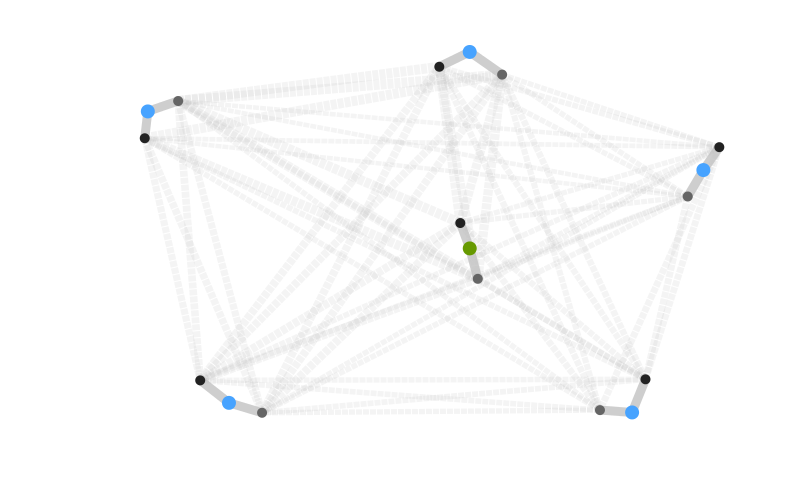
\includegraphics[width=1\columnwidth]{figures/graphseen.png}
    \caption{Graph representation of a scenario with 6 APs and 2 modules each. The grey eges indicate possible connectivity between the 
    modules. Edge weight(SNR) is mapped to edge thickness.}
    \label{fig:graphseen}
  \end{figure}
\section{Topology Creation}
  \subsection{Minimal/Optimal Spanning Tree Topology}
  In order to select those edges we want to use for creating connections between the APs, we use a derivation of the dijkstra algorithm. (cite dijkstra)
  We start by selecting an arbitray initial node and marking it as visited. All edges from this set of visited nodes to unvisited nodes are called productive edges.
  We keep those productive edges in a list sorted by their scores. The score of an edge is determined by the following formula:
  \begin{equation} \label{eq:edgescore}
    ES=\frac{b}{(i + 1 )* c}
  \end{equation}
  where \textit{ES} is the Score of this Edge, \textit{b} is the expected bandwidth, \textit{i} is the number of interfering modules and \textit{c} is the connected count of the corresponding nodes.
  \begin{description}
    \item[Expected Bandwidth]
    describes the expected available bandwidth we assume to get for this link depending on the Signal-to-Noise-Ratio.
    For a given Signal-to-Noise-Ratio we can estimate the maximal possible thoughput.
    The bandwidth was chosen as the numerator, since it is effectively shared by those the radio modules within range.
    As we can see from the diagram, a higher SNR value results in more bandwidth available and works in favor of this edge.
    \item[Connected Count]
    Number of nodes we can reach from Module A and Module B by just using module-module edges. 
    A higher connected count diminishes the importance of this edge, since this value controls how many channels we can use later for the overall graph.
    If this value would not be taken into consideration for calculating the score, the algorithm would rather create long chains of connected modules. 
    Those links in this chain would admittedly have the best SNR values, but since they have to share the same channel, it would result in lowering the overall throughput.
    Granting this value a higher impact in the formula, like for example in 
    \begin{equation}
      ES=\frac{b}{(i + 1)* c^2}
    \end{equation}
    , would have the effect of overemphasizing 
    the channel distribution and lead to poor choices in links with respect to SNR - lowering overall throughput again.
    This simple, linear impact in the formula has been shown to achieve the best tradeoff between those two extremes.
    \item[Interfering Modules]
    Since the channel assignment has not taken place yet, we do not know which modules are actually interfering with this link if we would use it.
    However we do know to which other modules this module already has connections to and since those have to use the same channel in order to communicate with each
    other, we can derive an estimate as lower bound for the number of interfering modules for this link (A,B) by counting the following modules:
    Total Interfering Modules = Number of visited nodes which we can reach by one hop over a module-module connection from node A and B
    . Those modules definetly interfer with our current connection, since they:
      are in range with at least one node of this connection (one hop distance)
      have to use the same channel (communication over module-module link)
      do actually interfere, because we already decided to use this connection (visited node)
    The value is incremented by one, because if this connection would be used, itself again acts as a source for interference.
    With an increasing count in interfering modues, the value of the link decreases and vice versa. This reflects perfectly the concept of a shared medium.
  \end{description}
  For each round we determine from this list the edge with the highest score and mark the new node as visited and add also the new links to the list.
  Finally we have to update the scores for each affected link and continue with the next round until all nodes are marked visited.
  The outcome is a minimal spanning tree for this graph with a custom evaluation function.
  \subsection{Survival Path}
  A spanning tree is very susceptible to graph partition by just removing or failing one link so we have to add redundancies in form of supplementary connections.
  However those redundant connections have to be carefully chosen in order not to negatively impact the successive channel assignment and neither to push interference.
  We accomplish this by iterating over all the edges of the spanning tree and simulate each connection failing. We then check if there still exists 
  a path from Node A to Node B of this failing connection. Only if this failing connection cuts the graph in half and there is no path to the other side,
  we start looking for a backup route in the following fashion:
  First we separate the the graph into two groups: Group A with all nodes and links reachable from Node A and Group B the same for Node B.
  We create a list with unused edges which connect the two groups and calculate the scores on them and pick again the edge with the highest score.
  This edge is, considering to the formula, the best edge to reconnect the two parts is called the survival edge for this scenario.
  Nevertheless we have to be aware that it might not be feasible to reconnect those parts if the underlying structure does not permit it.
  For example if the link between nodes \(E\) and \(F\) in \ref{fig:survival_algo} might be the only connection possible and failing it would cause network disruption.
  This results in a robust network topology, which despite the added interfering links still yields a high overall throughput with redundant paths.
  \begin{figure}[h]
    \centering
    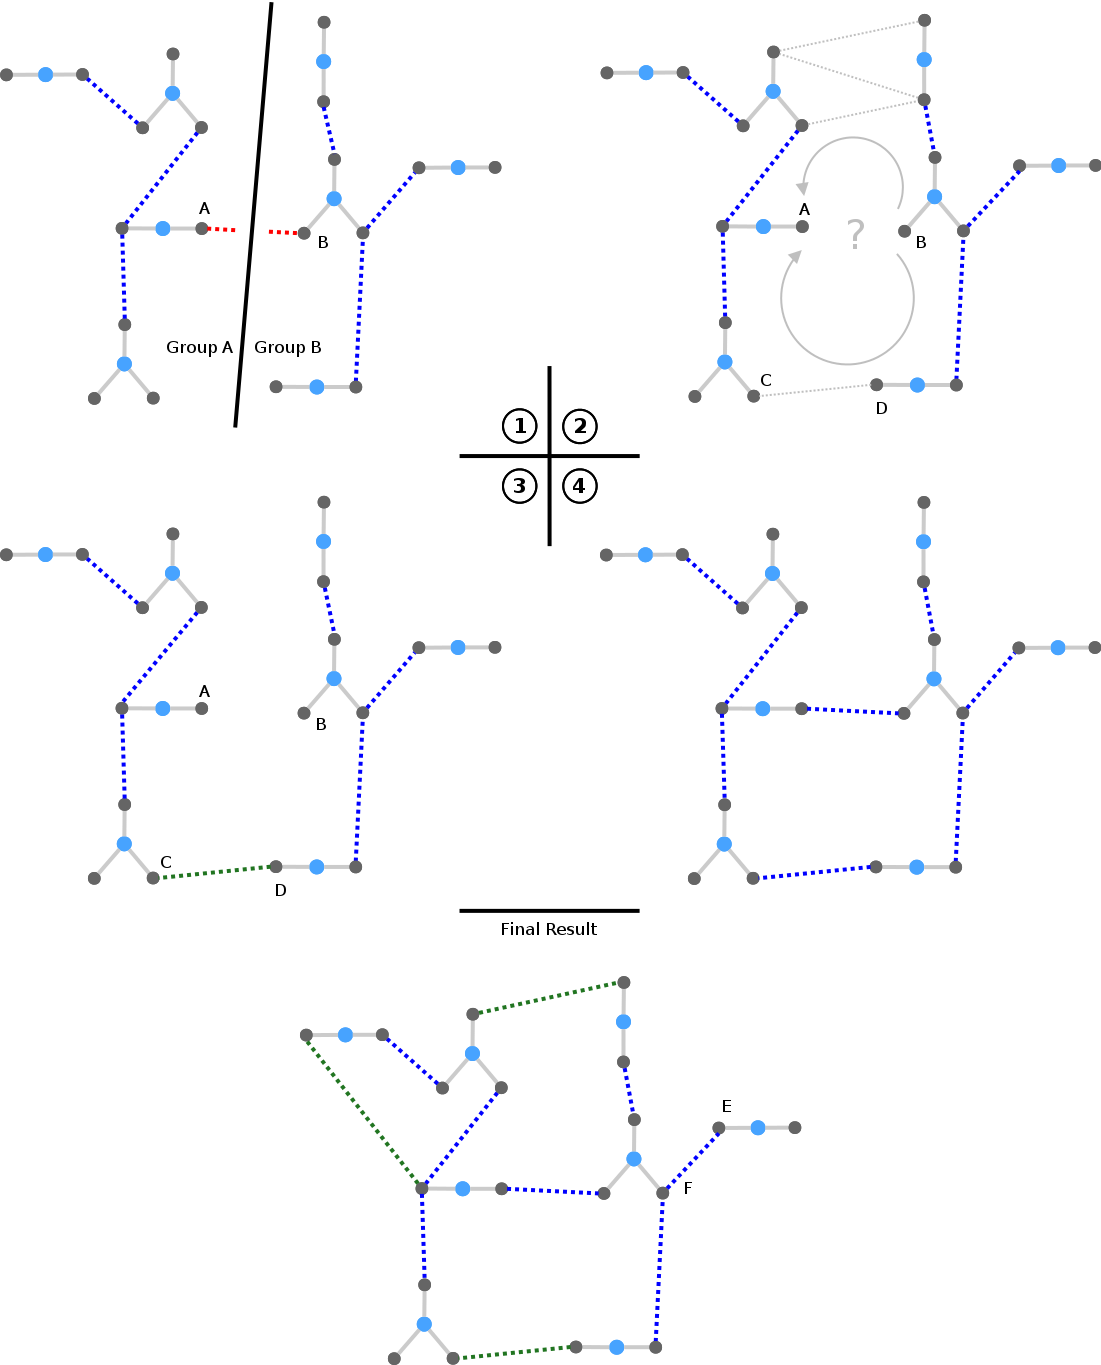
\includegraphics[width=1\columnwidth]{figures/survival_algo2}
    \caption{Finding survival paths. Simulation of connection between node A and node B failing, creating two groups.
    Finding a survival path for node A and B. Eventually all connections have a survival path. Here no redundant link possible for failing connection E,F.}
    \label{fig:survival_algo}
  \end{figure}
  The survival path attribute for a graph can be expressed ind the following way:
  For each edge (a,b) of the calculated spanning tree graph G', find a path from a to b without traversing (a,b), 
  in a way that the the sum of the Edgescores of the path is maximal.

\section{Channel Assignment Algorithm}
  For a given network topology graph and a set of channel to chose from, we can now assign channels to the module-nodes or if you like the links
  between those. Therefore we iterate over all module-module edges and assign channels to the adjacent module-nodes if they do not already have one assigned.
  The channel for an edge is chosen by the following pattern for each channel-group:
  Select all the modules which are connected by module-module edges. This set of nodes is called the channel-group.
  For this channel group we create a list of channels and corresponding interference occurrences.
  Among these we pick those channels from the set of all possible channels, which have been used the least in this channel-list. If there is a tie in usage
  we can also respect foreign networks by taking the occurrences of foreign radio modules into account or as a last resort-tie-breaker select one at random.
  Especially respecting foreign networks allows use to evade heavily used
  bands and channels like for example 1 and 11 in the 2.4Ghz band which are used by devices out of our control.
  \begin{figure}[h]
    \centering
    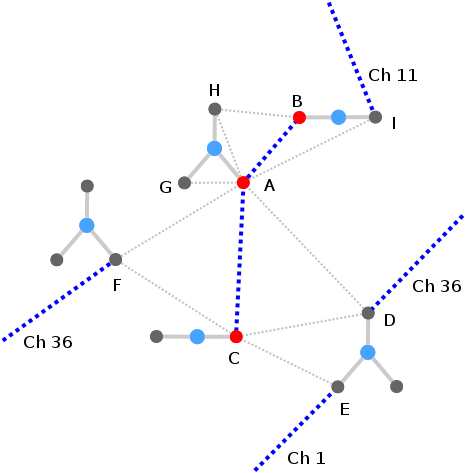
\includegraphics[width=1\columnwidth]{figures/channel-list}
    \caption{Assigning channels to the channel-set for nodes A,B,C. Since A,B and C are in the receive range of D,E,F,G,H,I they are possible sources
    of interference if we use the same channel as those. Therefore we survey how often every channel interferes, where one module can also interfere multiple times.
    For example does module F which already has channel 36 assigned interfere 4 times with the channel-set A,B,C ((A,F),(C,F),(C,D),(A,D)). If we only could choose from 
    channel 1,11 and 36 we would then decide to use Channel 1 or 11 to assign to the channel-set depending on how often we overall used those already.
    If however we want to take foreign networks into our consideration and lets say modules A and C would both detect two other \ac{WLAN} networks at channel 11 and two
    at channel 1, then we would add another 4 for channel 11 and 1 in the channel-list, leading to Channel 36 as the best choice. Note modules G and H are ignored 
    for the counting process since they do not have links or channels assigned.}
    \label{fig:channel-list}
  \end{figure}
  
  \begin{table}
    \centering
    \begin{tabular}{|c|c|}\hline
      Channel & Interference Count\\ \hline
      36 & 4 \\ \hline
      11 & 1 \\ \hline
      1 & 1 \\\hline
%      \caption{Channel-list without foreign influence}
    \end{tabular}
    \begin{tabular}{|c|c|}\hline
      Channel & Interference Count\\ \hline
      36 & 4 \\ \hline
      11 & 5 \\ \hline
      1 & 5  \\\hline
%      \caption{Channel-list with foreign influence}
    \end{tabular}
    \caption{Channel-list without (left) and with (right) foreign influence}
  \end{table}
 
  \begin{figure}[h]
    \centering
    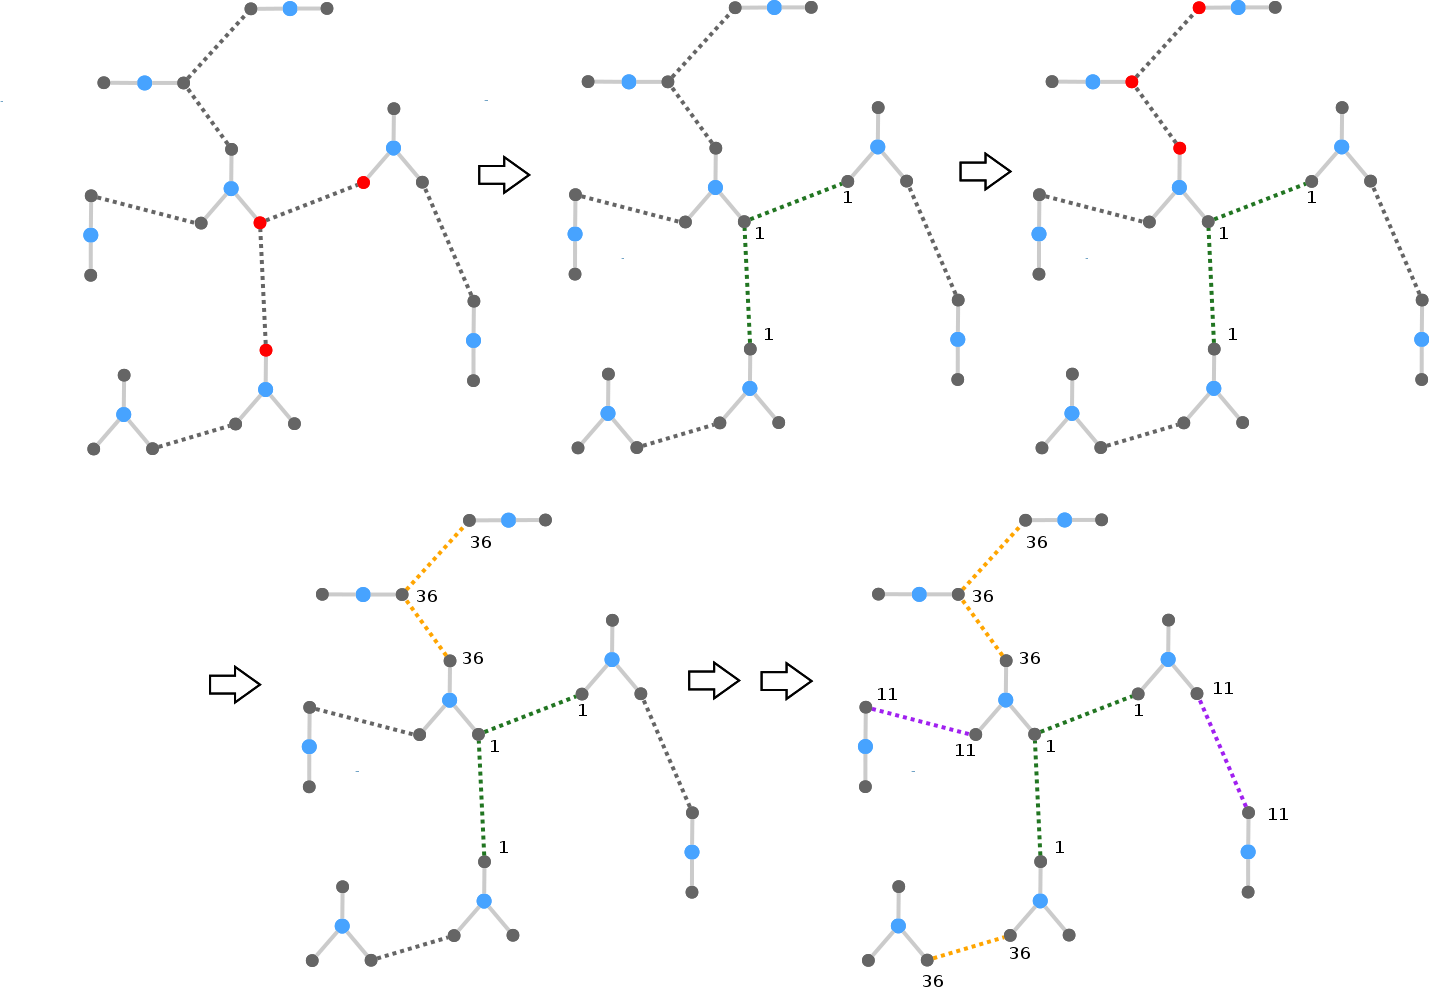
\includegraphics[width=1\columnwidth]{figures/caa_algo}
    \caption{Bigger picture channel assignment showing the results after each assingment to the channel-groups. 
    Example-assignment for a network with 8 Accesspoints with 2 and 3 modules equipped and available channels [1,11,36] without foreign influence. 
    The first four graphs represent the first 4 rounds. Red marked nodes represent a channel-group.}
    \label{fig:caa_algo}
  \end{figure}
